% Pipeline usulan Fase 2: mesin OCR sebagai variabel + dua cara fusi.
% Kompilasi: latexmk -pdf main.tex
\documentclass[border=8pt]{standalone}
\usepackage[T1]{fontenc}
\usepackage[sfdefault,lining]{carlito}
\usepackage{tikz}
\usetikzlibrary{arrows.meta,positioning,fit,calc,backgrounds}
\begin{document}
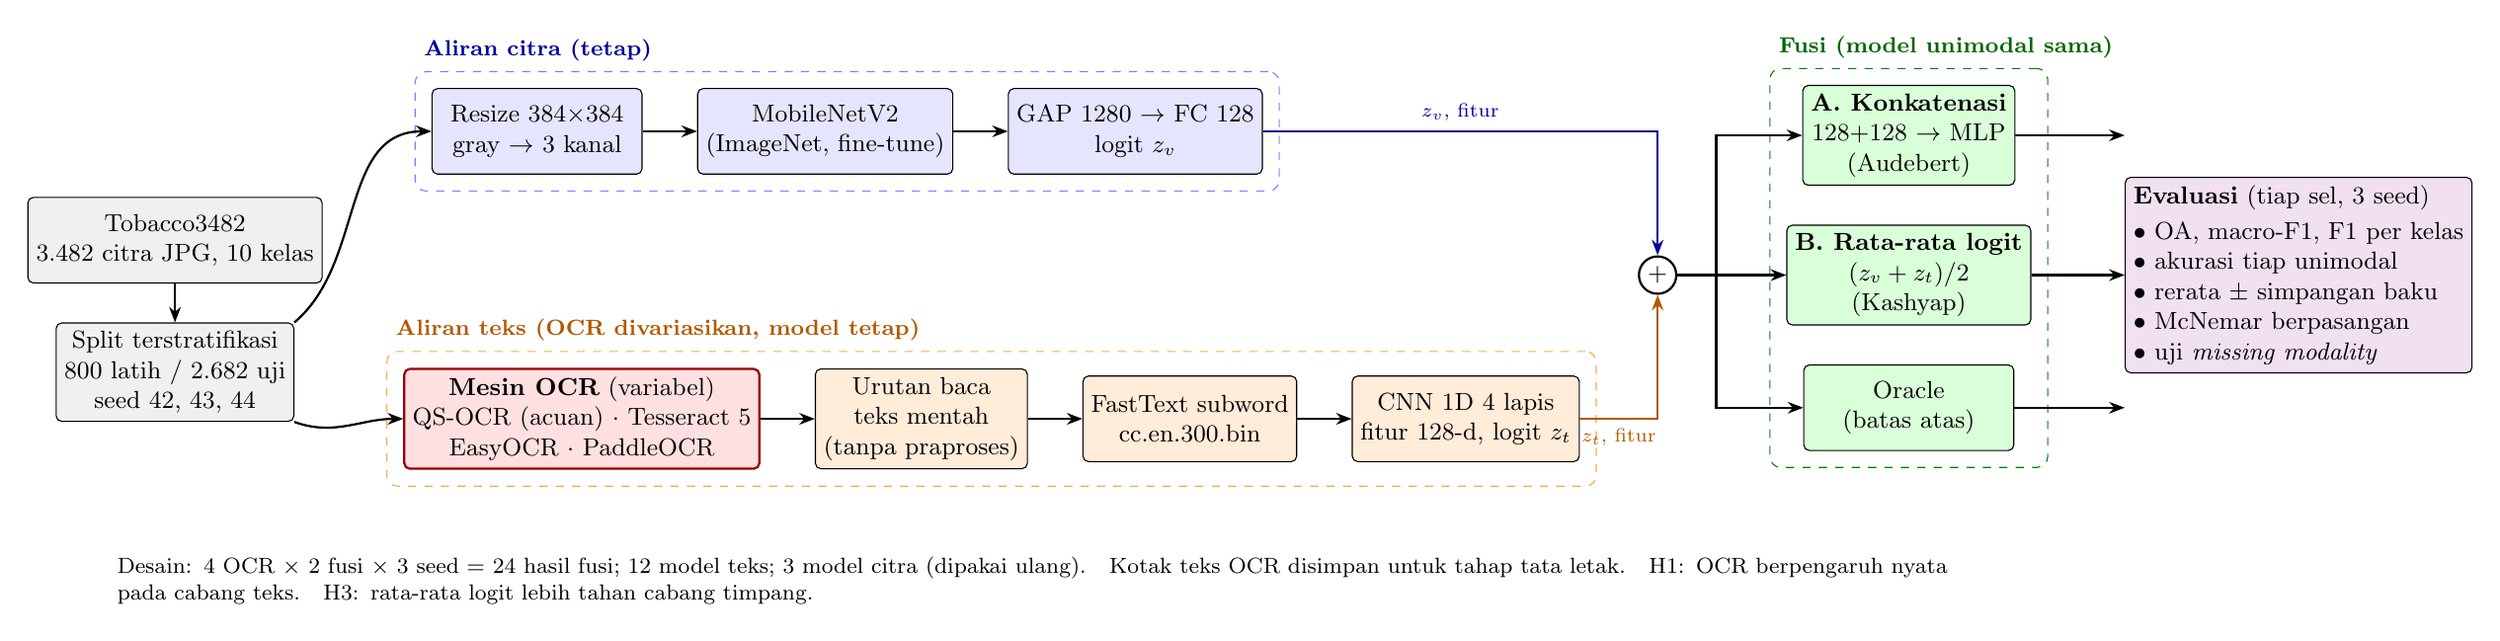
\begin{tikzpicture}[
  node distance=5mm and 7mm,
  kotak/.style={draw, rounded corners=2pt, align=center, font=\small,
                minimum height=11mm, minimum width=27mm, inner sep=3pt},
  data/.style={kotak, fill=gray!12},
  citra/.style={kotak, fill=blue!10},
  teks/.style={kotak, fill=orange!15},
  var/.style={kotak, fill=red!12, draw=red!60!black, thick},
  fusi/.style={kotak, fill=green!15},
  eval/.style={kotak, fill=violet!12},
  grup/.style={draw, dashed, rounded corners=4pt, inner sep=6pt},
  label/.style={font=\footnotesize\bfseries, anchor=south west},
  panah/.style={-{Stealth[length=2mm]}, thick}]

  % ---- data
  \node[data] (data) {Tobacco3482\\3.482 citra JPG, 10 kelas};
  \node[data, below=of data] (split) {Split terstratifikasi\\800 latih / 2.682 uji\\seed 42, 43, 44};
  \draw[panah] (data) -- (split);

  % ---- aliran citra
  \node[citra, right=14mm of data, yshift=14mm] (rs) {Resize 384$\times$384\\gray $\to$ 3 kanal};
  \node[citra, right=of rs] (mb) {MobileNetV2\\(ImageNet, fine-tune)};
  \node[citra, right=of mb] (fv) {GAP 1280 $\to$ FC 128\\logit $z_v$};

  % ---- aliran teks
  \node[var, right=14mm of split, yshift=-6mm] (ocr) {\textbf{Mesin OCR} (variabel)\\QS-OCR (acuan) $\cdot$ Tesseract 5\\EasyOCR $\cdot$ PaddleOCR};
  \node[teks, right=of ocr] (ro) {Urutan baca\\teks mentah\\(tanpa praproses)};
  \node[teks, right=of ro] (ft) {FastText subword\\cc.en.300.bin};
  \node[teks, right=of ft] (cnn) {CNN 1D 4 lapis\\fitur 128-d, logit $z_t$};

  \draw[panah] (split.north east) to[out=40,in=180] (rs.west);
  \draw[panah] (split.south east) to[out=-20,in=180] (ocr.west);
  \draw[panah] (rs) -- (mb); \draw[panah] (mb) -- (fv);
  \draw[panah] (ocr) -- (ro); \draw[panah] (ro) -- (ft); \draw[panah] (ft) -- (cnn);

  % ---- fusi: kedua aliran bertemu di satu titik, lalu ke tiga kotak fusi
  \node[circle, draw, thick, fill=white, inner sep=1.5pt, font=\small]
    (j) at ($(cnn.east |- {$(fv)!0.5!(cnn)$})+(10mm,0)$) {$+$};
  \draw[panah, blue!60!black] (fv.east) -| node[pos=0.25, above, font=\scriptsize] {$z_v$, fitur} (j.north);
  \draw[panah, orange!70!black] (cnn.east) -| node[pos=0.25, below, font=\scriptsize] {$z_t$, fitur} (j.south);
  \node[fusi, right=14mm of j] (fb) {\textbf{B. Rata-rata logit}\\$(z_v+z_t)/2$\\(Kashyap)};
  \node[fusi, above=of fb] (fa) {\textbf{A. Konkatenasi}\\128+128 $\to$ MLP\\(Audebert)};
  \node[fusi, below=of fb] (or) {Oracle\\(batas atas)};
  \foreach \n in {fa,fb,or} \draw[panah] (j.east) -- ++(5mm,0) |- (\n.west);

  % ---- evaluasi
  \node[eval, right=12mm of fb, minimum width=40mm, align=left] (ev) {\textbf{Evaluasi} (tiap sel, 3 seed)\\[2pt]
    $\bullet$ OA, macro-F1, F1 per kelas\\
    $\bullet$ akurasi tiap unimodal\\
    $\bullet$ rerata $\pm$ simpangan baku\\
    $\bullet$ McNemar berpasangan\\
    $\bullet$ uji \emph{missing modality}};
  \draw[panah] (fa.east) -- (ev.west |- fa.east);
  \draw[panah] (fb.east) -- (ev.west);
  \draw[panah] (or.east) -- (ev.west |- or.east);

  % ---- kelompok
  \begin{scope}[on background layer]
    \node[grup, draw=blue!50, fit=(rs)(mb)(fv)] (gc) {};
    \node[grup, draw=orange!70, fit=(ocr)(ro)(ft)(cnn)] (gt) {};
    \node[grup, draw=green!50!black, fit=(fa)(fb)(or)] (gf) {};
  \end{scope}
  \node[label, text=blue!60!black] at (gc.north west) {Aliran citra (tetap)};
  \node[label, text=orange!70!black] at (gt.north west) {Aliran teks (OCR divariasikan, model tetap)};
  \node[label, text=green!40!black] at (gf.north west) {Fusi (model unimodal sama)};

  % ---- catatan kaki
  \node[font=\footnotesize, align=left, anchor=north west, text width=24cm]
    at ($(ocr.south west)+(-38mm,-10mm)$)
    {Desain: 4 OCR $\times$ 2 fusi $\times$ 3 seed = 24 hasil fusi; 12 model teks; 3 model citra (dipakai ulang).\quad
     Kotak teks OCR disimpan untuk tahap tata letak.\quad
     H1: OCR berpengaruh nyata pada cabang teks.\quad
     H3: rata-rata logit lebih tahan cabang timpang.};
\end{tikzpicture}
\end{document}
